\setcounter{section}{0}

\section{Lý thuyết}
\subsection{Chuyển động tròn}
Chuyển động tròn là một trong những loại chuyển động ta thường thấy trong đời sống: một điểm trên cánh quạt chuyển động theo một đường tròn khi cánh quạt quay, chuyển động của một vệ tinh nhân tạo xung quanh Trái Đất.

\textbf{Định nghĩa.} Chuyển động tròn là chuyển động có quỹ đạo là một đường tròn.
\begin{center}
	
\includegraphics[scale=0.3]{../figs/VN10-PH-06-L-005-1-V2-01.jpg}
\end{center}
\subsection{Tốc độ trung bình trong chuyển động tròn}

\textbf{Định nghĩa.} Tốc độ trung bình trong chuyển động tròn là độ dài cung tròn mà vật đi được trong một đơn vị thời gian.
\begin{center}
	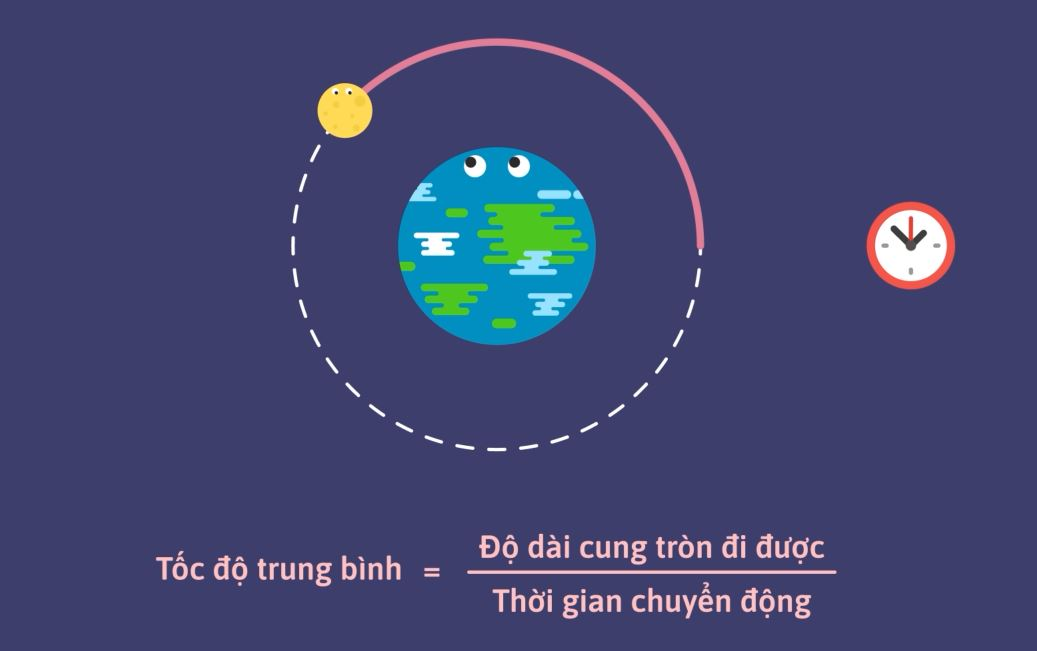
\includegraphics[scale=0.3]{../figs/VN10-PH-06-L-005-1-V2-02.jpg}
\end{center}
\subsection{Chuyển động tròn đều}
Chuyển động tròn đều là chuyển động có quỹ đạo tròn và có tốc độ trung bình không đổi trên mọi cung tròn của quỹ đạo. 

\begin{center}
	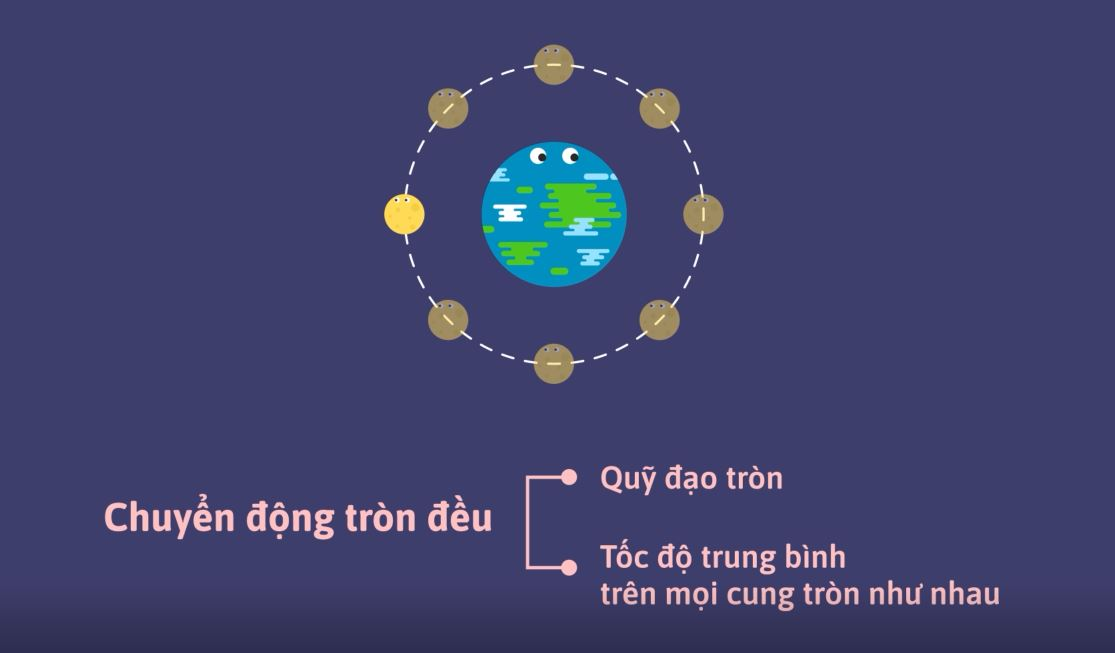
\includegraphics[scale=0.3]{../figs/VN10-PH-06-L-005-1-V2-03.jpg}
\end{center}
\subsection{Độ dịch chuyển góc}
Giả sử một vật chuyển động trên một đường tròn bán kính $r$. Trong thời gian $\Delta t$ vật đi được quãng đường $\Delta s$. Góc $\Delta \alpha$ ứng với cung tròn $\Delta s$ mà vật đã đi được kể từ vị trí ban đầu gọi là độ dịch chuyển góc:
$$\Delta \alpha = \dfrac{\Delta s}{r}$$

Đơn vị của độ dịch chuyển góc là rad.
\luuy{Trong Vật lí người ta thường đo góc theo đơn vị radian (kí hiệu rad), với $\SI{1}{rad}$ là số đo góc ở tâm một đường tròn chắn cung có độ dài bằng bán kính đường tròn đó.
	$$\SI{1}{rad} = \dfrac{180^\circ}{\pi} = \dfrac{180^\circ}{\SI{3.1416}{}\ldots} \approx\SI{57.2958}{^\circ}$$
	\begin{center}
		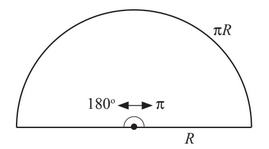
\includegraphics{../figs/G10-026-1}
	\end{center}
}
\subsection{Tốc độ góc và tốc độ dài trong chuyển động tròn}
\subsubsection{Tốc độ góc}
\textbf{Định nghĩa.} Tốc độ góc trong chuyển động tròn có giá trị bằng độ dịch chuyển góc trong một đơn vị thời gian:
$$\omega = \frac{\Delta \alpha}{\Delta t}$$

Đơn vị của tốc độ góc trong hệ đơn vị SI là $\SI{}{\radian/\second}$.\\

Trong chuyển động tròn đều, tốc độ góc của vật không đổi. 
\begin{center}
	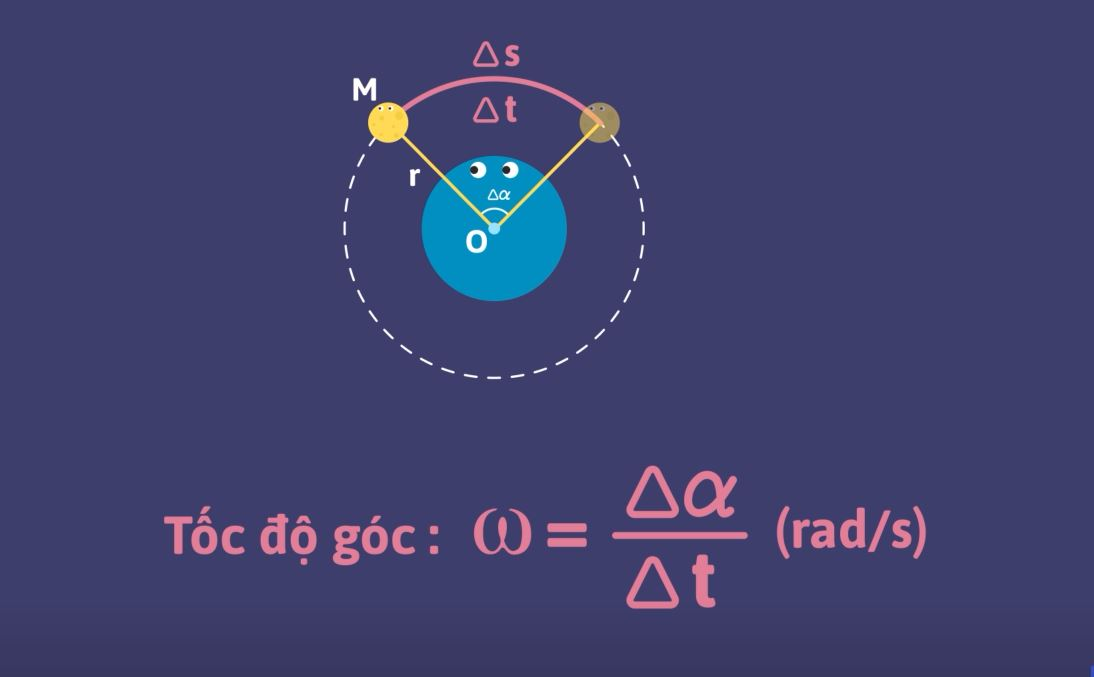
\includegraphics[scale=0.3]{../figs/VN10-PH-06-L-005-2-V2-02.jpg}
\end{center}
\subsubsection{Tốc độ dài}
Trong chuyển động tròn, mỗi điểm trên bán kính đều có cùng tốc độ góc, nhưng vì mỗi điểm này có thể có quãng đường chuyển động khác nhau nên để phân biệt với tốc độ góc, ta sử dụng khái niệm tốc độ dài.

\textbf{Định nghĩa.} Tốc độ dài (gọi tắt là là tốc độ) của một chất điểm chuyển động tròn được tính bằng quãng đường mà chất điểm di chuyển được trong một đơn vị thời gian:
$$v=\frac{\Delta s}{\Delta t} $$

Đơn vị của tốc độ dài trong hệ đơn vị SI là $\SI{}{\meter/\second.}$.\\

Trong chuyển động tròn đều, tốc độ dài của vật không đổi. \\
\begin{center}
	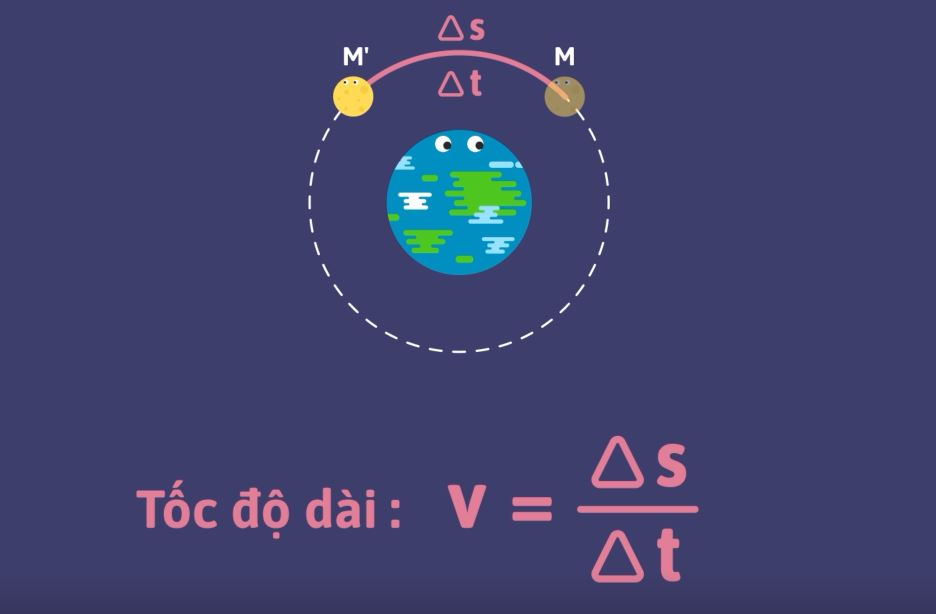
\includegraphics[scale=0.3]{../figs/VN10-PH-06-L-005-2-V2-01.jpg}
\end{center}	

\begin{minipage}{0.6\textwidth}
	Khi nói về phương, chiều của tốc độ dài, người ta sử dụng khái niệm vectơ vận tốc (gọi tắt là vận tốc). Vận tốc trong chuyển động tròn có phương tiếp tuyến với đường tròn quỹ đạo và có chiều là chiều của chuyển động.
	
	Trong chuyển động tròn đều, độ lớn của vận tốc tức thời không đổi nhưng hướng luôn thay đổi.
\end{minipage}
\begin{minipage}{0.4\textwidth}
	\begin{center}
		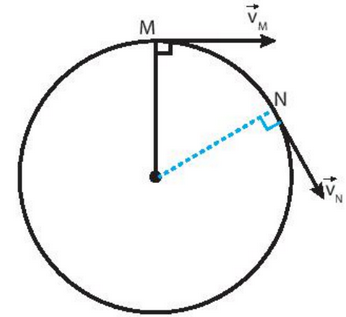
\includegraphics[scale=0.6]{../figs/G10-026-2}
	\end{center}
\end{minipage}


\subsubsection{Liên hệ giữa tốc độ góc và tốc độ dài}
Công thức liên hệ giữa tốc độ góc và tốc độ dài:
$$v=r\omega,$$ 
trong đó, $r$ là bán kính quỹ đạo tròn.		


\subsection{Chu kì và tần số}
Ngoài tốc độ, tốc độ góc, trong chuyển động tròn đều người ta còn quan tâm đến các đại lượng như chu kì và tần số.

\subsubsection{Chu kì}

Chu kì (kí hiệu là $T$) trong chuyển động tròn đều là thời gian để vật đi được một vòng tròn.

\subsubsection{Tần số}
Tần số (kí hiệu là $f$) là số vòng vật đi được trong một giây.

Đơn vị tần số là hertz (Hz).

\subsubsection{Liên hệ giữa chu kì, tần số, và tốc độ góc}

Công thức liên hệ giữa chu kì, tần số và tần số góc:

$$T=\dfrac{1}{f}=\dfrac{2\pi}{\omega},$$
trong đó, $T$ là chu kì, $f$ là tần số, $\omega$ là tốc độ góc. 				


\section{Mục tiêu bài học - Ví dụ minh họa}
\begin{dang}{Nhận biết đặc điểm của  chuyển động tròn đều}
	\viduii{1}{Chuyển động nào dưới đây là chuyển động tròn đều?
		\begin{mcq}
			\item Chuyển động của mắt xích xe đạp khi xe chạy.
			\item Chuyển động của đầu cánh quạt trần khi quay ổn định.
			\item Chuyển động của đầu cánh quạt trần khi vừa bật.
			\item Chuyển động của con lắc đồng hồ.
		\end{mcq}
	}
	{	\begin{center}
			\textbf{Hướng dẫn giải}
		\end{center}
		
		Chuyển động tròn đều là chuyển động có các đặc điểm:
		\begin{itemize}
			\item Quỹ đạo là một đường tròn;
			\item Tốc độ trung bình trên mọi cung tròn là như nhau.
		\end{itemize}
		Chuyển động A không thỏa điều kiện quỹ đạo tròn. Chuyển động C không thỏa điều kiện tốc độ trung bình như nhau. Chuyển động D không thỏa điều kiện tốc độ trung bình như nhau. Chuyển động B thỏa mãn cả hai điều kiện. 
		
		\textbf{Đáp án: B}.
		
	}
	\viduii{1}{Chuyển động của vật nào dưới đây là chuyển động tròn đều?
		\begin{mcq}
			\item Chuyển động của đầu van bánh xe đạp khi xe đang chuyển động thẳng chậm dần đều.
			\item Chuyển động quay của Trái Đất quanh Mặt Trời.
			\item Chuyển động của điểm đầu cánh quạt trần khi đang quay ổn định.
			\item Chuyển động của điểm đầu cánh quạt khi vừa tắt điện.
		\end{mcq}
	}
	{	\begin{center}
			\textbf{Hướng dẫn giải}
		\end{center}
		Chuyển động A không thỏa điều kiện về tốc độ trung bình không đổi. \\
		Chuyển động B không thỏa mãn quỹ đạo tròn (quỹ đạo của Trái đất quanh Mặt trời là một đường ê-líp gần tròn).\\
		Chuyển động D là chuyển động chậm dần, không thỏa điều kiện về tốc độ trung bình không đổi. 
		
		\textbf{Đáp án: C}.
	}
	
\end{dang}
\begin{dang}{Biểu diễn đơn vị độ dịch chuyển góc}
	\viduii{2}{Đổi các góc sau từ độ sang radian: $30^\circ$, $90^\circ$.
	}
	{	\begin{center}
			\textbf{Hướng dẫn giải}
		\end{center}
		
		Ta có:
		$$x^\circ \longrightarrow \dfrac{x \pi}{180}\ \text{rad}.$$
		
		Đổi $$30^\circ \longrightarrow \dfrac{30\pi}{180}\ \text{rad} = \dfrac{\pi}{6}\ \text{rad}$$
		
		Đổi $$90^\circ \longrightarrow \dfrac{\SI{90}{\degree}\pi}{\SI{180}{\degree}}\ \text{rad} = \dfrac{\pi}{2}\ \text{rad}$$
		
		\begin{center}
			\textbf{Câu hỏi tương tự}
		\end{center}
		
		Đổi các góc sau từ độ sang radian: $105^\circ$, $120^\circ$, $270^\circ$.
		
		\textbf{Đáp án:} $105^\circ \longrightarrow \dfrac{7\pi}{12}\ \text{rad}$; $120^\circ \longrightarrow \dfrac{2\pi}{3}\ \text{rad}$; $270^\circ \longrightarrow \dfrac{3\pi}{22}\ \text{rad}$.
	}
	\viduii{2}{Đổi các góc sau từ radian sang độ: $\SI{0.25}{rad}$, $\SI{0.5}{rad}$.
	}
	{	\begin{center}
			\textbf{Hướng dẫn giải}
		\end{center}
		
		Ta có:
		$$x\ \text{rad} \longrightarrow \left(\dfrac{x \cdot 180}{\pi}\right)^\circ.$$
		
		Đổi $$\SI{0.25}{rad} \longrightarrow \dfrac{0,25 \cdot \SI{180}{\degree}}{\pi} = 14,33^\circ$$
		
		Đổi $$\SI{0.5}{rad} \longrightarrow \dfrac{0,5 \cdot \SI{180}{\degree}}{\pi} = 28,66^\circ$$
		
		\begin{center}
			\textbf{Câu hỏi tương tự}
		\end{center}
		
		Đổi các góc sau từ radian sang độ: $\xsi{0,5\pi}{rad}$, $\xsi{\pi}{rad}$.
		
		\textbf{Đáp án:} $\xsi{0,5\pi}{rad} \longrightarrow 90^\circ$; $\xsi{\pi}{rad} \longrightarrow 180^\circ$.
	}
\end{dang}
\begin{dang}{Tính tốc độ dài, tốc độ góc, chu kỳ, tần số trong chuyển động tròn đều}
	\viduii{2}{Một vệ tinh nhân tạo bay quanh Trái Đất theo một quỹ đạo tròn. Chu kì của vệ tinh là $88\ \text{phút}$. Tính tốc độ góc của vệ tinh. 
	}
	{	\begin{center}
			\textbf{Hướng dẫn giải}
		\end{center}
		Tốc độ góc của vệ tinh:
		$$T=\frac{2\pi}{\omega} \quad\Rightarrow\quad \omega = \frac{\pi}{2640}\ \text{rad/s}.$$ 
		
		\begin{center}
			\textbf{Câu hỏi tương tự}
		\end{center}
		
		Roto trong một tổ máy của nhà máy thủy điện Hòa Bình quay 125 vòng mỗi phút. Hãy tính tốc độ góc của roto này theo đơn vị rad/s.
		
		\textbf{Đáp án:} $\omega \approx \SI{13.1}{rad/s}$.
	}
	
	\viduii{3}{
		Kim phút của đồng hồ dài gấp 1,5 lần kim giờ. Hỏi tốc độ dài của đầu kim phút lớn gấp mấy lần tốc độ dài của đầu kim giờ?
	}
	{	\begin{center}
			\textbf{Hướng dẫn giải}
		\end{center}
		
		Gọi $\omega_1, \omega_2$ lần lượt là tốc độ góc của kim phút và kim giờ. Kim phút quay một vòng ($2\pi\ \SI{}{\radian}$) trong 1 giờ, kim giờ quay một vòng trong 12 giờ, do đó 
		$$
		\dfrac{\omega_1}{\omega_2}=12
		$$
		
		Ta lập được tỉ số: $$\dfrac{v_1}{v_2}=\dfrac{\omega_1 \cdot R_1}{\omega_2 \cdot R_2}=\dfrac{\omega_1}{\omega_2}\cdot\dfrac{R_1}{R_2}=18.$$
		
		\begin{center}
			\textbf{Câu hỏi tương tự}
		\end{center}
		
		Biết chiều dài kim phút và kim giây của một chiếc đồng hồ lần lượt là $\SI{4}{cm}$ và $\SI{5}{cm}$. Hãy tính:
		\begin{enumerate}[label=\alph*)]
			\item Tỉ số chu kì quay của hai kim.
			\item Tỉ số tốc độ của đầu kim phút và đầu kim giây.
		\end{enumerate}
		
		\textbf{Đáp án:}
		\begin{enumerate}[label=\alph*)]
			\item $\frac{T_\text{phút}}{T_\text{giây}}=60$.
			\item $\frac{v_\text{phút}}{v_\text{giây}}=\dfrac{1}{75}$.
		\end{enumerate}
	}
	
	
	
\end{dang}
\section{Trắc nghiệm}
\begin{enumerate}[label=\bfseries Câu \arabic*:]
	\item \mkstar{2}
	
	
	{
		Chuyển động của vật nào dưới đây được coi là chuyển động tròn đều?
		\begin{mcq}
			\item Chuyển động của bánh xe ô tô khi đang hãm phanh.
			\item Chuyển động của kim phút trên mặt đồng hồ chạy đúng giờ.
			\item Chuyển động quay của các điểm treo các ghế ngồi trên chiếc đu quay.
			\item Chuyển động quay của cánh quạt khi vừa tắt điện.
		\end{mcq}
	}
	
	\hideall
	{	
		\textbf{Đáp án: B.}
		
		Chuyển động của kim phút trên mặt đồng hồ chạy đúng giờ là chuyển động tròn đều.
	}
	\item \mkstar{2}
	
	
	{
		Các công thức liên hệ giữa tốc độ góc $\omega$ với chu kỳ $T$ và giữa tốc độ góc $\omega$ với tần số $f$ trong chuyển động tròn đều là gì?
		\begin{mcq}(2)
			\item $\omega=2\pi T$; $\omega=\dfrac{2\pi}{f}$.
			\item $\omega=\dfrac{2\pi}{T}$; $\omega=2\pi f$.
			\item $\omega=2\pi T$; $\omega=2\pi f$. 
			\item $\omega=\dfrac{2\pi}{T}$; $\omega=\dfrac{2\pi}{f}$.
		\end{mcq}
	}
	
	\hideall
	{	
		\textbf{Đáp án: B.}
		
		Công thức liên hệ giữa tốc độ góc $\omega$ với chu kỳ $T$ là $\omega=\dfrac{2\pi}{T}$.
		Công thức liên hệ giữa giữa tốc độ góc $\omega$ với tần số $f$ trong chuyển động tròn đều là $\omega=2\pi f$.
	}
	\item \mkstar{2}
	
	
	{
		Một bánh xe có đường kính $\SI{100}{\centi\meter}$ lăn đều với vận tốc $\SI{36}{\kilo\meter/\hour}$. Gia tốc hướng tâm của một điểm trên vành bánh xe có độ lớn
		\begin{mcq}(4)
			\item $\SI{200}{\meter/\second^2}$.
			\item $\SI{400}{\meter/\second^2}$.
			\item $\SI{100}{\meter/\second^2}$.
			\item $\SI{300}{\meter/\second^2}$.
		\end{mcq}
	}
	
	\hideall
	{	
		\textbf{Đáp án: A.}
		
		Đổi đơn vị: $\SI{100}{\centi\meter}=\SI{1}{\meter}$; $\SI{36}{\kilo\meter/\hour}=\SI{10}{\meter/\second}$
		
		Gia tốc hướng tâm của một điểm trên vành bánh xe có độ lớn:
		$$a_\text{ht}=\dfrac{v^2}{R}=\SI{200}{\meter/\second^2}.$$
	}
	\item \mkstar{2}
	
	
	{
		Một đĩa tròn bán kính $\SI{20}{\centi\meter}$ quay đều quanh trục của nó. Đĩa quay hết 1 vòng mất $\SI{0.2}{\second}$. Tốc độ dài $v$ của một điểm nằm ở mép đĩa bằng
		\begin{mcq}(4)
			\item $\SI{4,71}{\meter/\second}$. 
			\item $\SI{3,14}{\meter/\second}$. 
			\item $\SI{6,28}{\meter/\second}$. 
			\item $\SI{7,85}{\meter/\second}$.
		\end{mcq}
	}
	
	\hideall
	{	
		\textbf{Đáp án: C.}
		
		Tốc độ dài $v$ của một điểm trên vành ngoài xe:
		$v=r\omega=r\dfrac{\Delta \alpha}{\Delta t}=\SI{0,2}{\meter}\dfrac{2\pi}{\SI{0.2}{\second}}=\SI{6,28}{\meter/\second}$
	}
	\item \mkstar{2}
	
	
	{
		Một động cơ xe máy có trục quay 1200 vòng/phút. Tốc độ góc của chuyển động quay là bao nhiêu?
		\begin{mcq}(4)
			\item $\SI{125,7}{\radian/\second}$.
			\item $\SI{188,5}{\radian/\second}$.
			\item $\SI{62,8}{\radian/\second}$.
			\item $\SI{7200}{\radian/\second}$.
		\end{mcq}
	}
	
	\hideall
	{	
		\textbf{Đáp án: A.}
		
		Tốc độ góc của chuyển động quay là:
		$\omega$ = 1200 vòng/ phút = $1200\cdot\dfrac{2\pi}{60}\,\SI{}{\radian/\second}=\SI{125,7}{\radian/\second}$
	}
	\item \mkstar{2}
	
	
	{
		Một bánh xe có bán kính $\SI{100}{\centi\meter}$ lăn đều với vận tốc $\SI{54}{\kilo\meter/\hour}$. Gia tốc hướng tâm của một điểm trên vành bánh xe có độ lớn
		\begin{mcq}(4)
			\item $\SI{225}{\meter/\second^2}$.
			\item $\SI{400}{\meter/\second^2}$.
			\item $\SI{100}{\meter/\second^2}$.
			\item $\SI{300}{\meter/\second^2}$.
		\end{mcq}
	}
	
	\hideall
	{	
		\textbf{Đáp án: A.}
		
		Gia tốc hướng tâm của một điểm trên vành bánh xe có độ lớn:
		$$a_\text{ht}=\dfrac{v^2}{R}=\SI{225}{\meter/\second^2}.$$
	}
	\item \mkstar{2}
	
	
	{
		Một vệ tinh nhân tạo ở độ cao $\SI{250}{\kilo\meter}$ bay quanh Trái Đất theo một quỹ đạo tròn. Chu kì của vệ tinh là 88 phút. Tính gia tốc hướng tâm của vệ tinh. Cho bán kính Trái Đất là $\SI{6400}{\kilo\meter}$.
		\begin{mcq}(4)
			\item $\SI{9,41}{ \meter/\second^2}$.
			\item $\SI{9,48}{ \meter/\second^2}$.
			\item $\SI{8,72}{ \meter/\second^2}$.
			\item $\SI{10,05}{ \meter/\second^2}$.
		\end{mcq}
	}
	
	\hideall
	{	
		\textbf{Đáp án: A.}
		
		Khoảng cách từ vệ tinh đến tâm Trái Đất: 
		$$r=\SI{250}{\kilo\meter}+\SI{6400}{\kilo\meter} =\SI{6650}{\kilo\meter}=\SI{6650000}{\meter}.$$
		
		Tốc độ góc của vệ tinh:
		$$T=\frac{2\pi}{\omega} \Rightarrow \omega = \frac{\pi}{2640}\ \text{rad/s}.$$ 
		
		Gia tốc hướng tâm của vệ tinh: 
		
		$$a_{ht}=\omega^2 \cdot r \approx \SI{9,41}{ \meter/\second^2}.$$
	}
	\item \mkstar{2}
	
	
	{
		Xe đạp của một vận động viên chuyển động thẳng đều với $v=\SI{36}{km/h}$. Biết bán kính của lốp xe đạp là $\SI{32.5}{cm}$. Tính tốc độ góc và gia tốc hướng tâm tại một điểm trên lốp bánh xe.
		\begin{mcq}(2)
			\item $\omega = \SI{30.77}{rad/s}$, $a_\text{ht} = \SI{307.7}{m/s^2}$.
			\item $\omega = \SI{30.77}{rad/s}$, $a_\text{ht} = \SI{377.7}{m/s^2}$.
			\item $\omega = \SI{3.77}{rad/s}$, $a_\text{ht} = \SI{30.7}{m/s^2}$.
			\item $\omega = \SI{3.77}{rad/s}$, $a_\text{ht} = \SI{307.7}{m/s^2}$.
		\end{mcq}
	}
	
	\hideall
	{	
		\textbf{Đáp án: A.}
		
		Vận tốc xe đạp cũng là tốc độ dài của một điểm trên lốp xe:
		$$v=\SI{36}{km/h} = \SI{10}{m/s}$$
		
		Tốc độ góc:
		$$\omega = \dfrac{v}{R} = \SI{30.77}{rad/s}$$
		
		Gia tốc hướng tâm:
		$$a_\text{ht} = \dfrac{v^2}{R} = \SI{307.7}{m/s^2}$$
	}
	\item \mkstar{2}
	
	
	{
		Hai vật A và B chuyển động tròn đều với cùng chu kì trên hai đường tròn có bán kính khác nhau lần lượt là $R_\text A$ và $R_\text B$, với $R_\text A = 4 R_\text B$. Nếu vật A chuyển động với tốc độ dài $\SI{12}{m/s}$ thì tốc độ dài của vật B là
		\begin{mcq}(4)
			\item $\SI{48}{m/s}$.
			\item $\SI{24}{m/s}$.
			\item $\SI{3}{m/s}$.
			\item $\SI{4}{m/s}$.
		\end{mcq}
	}
	
	\hideall
	{	
		\textbf{Đáp án: C.}
		
		Lập tỉ lệ:
		$$\dfrac{v_\text A}{v_\text B} = \dfrac{R_\text B}{R_\text A} = \dfrac{1}{4} \Rightarrow v_\text B =\SI{3}{m/s} $$
	}
	\item \mkstar{2}
	
	
	{
		Hai vật A và B chuyển động tròn đều trên hai đường tròn tiếp xúc nhau. Chu kì của A là 4 s, còn chu kì của B là 2 s. Biết rằng tại thời điểm ban đầu chúng xuất phát cùng một lúc từ điểm tiếp xúc của hai đường tròn và chuyển động ngược chiều nhau. Khoảng thời gian ngắn nhất để hai vật gặp nhau lần nữa là
		\begin{mcq}(4)
			\item $1\ \text s$.
			\item $2\ \text s$.
			\item $6\ \text s$.
			\item $4\ \text s$.
		\end{mcq}
	}
	
	\hideall
	{	
		\textbf{Đáp án: D.}
		
		Khoảng thời gian ngắn nhất để hai vật gặp nhau lần nữa:
		$$\Delta t = \dfrac{\Delta \varphi_\text A }{\omega_\text A} = \dfrac{\Delta \varphi_\text B }{\omega_\text B}$$
		
		Trong đó $\Delta \varphi_\text A = n \Delta \varphi_\text B$, với $n=2k$ với ($k\in Z$)
		
		Vậy khoảng thời gian ngắn nhất khi $n=2$, khi đó $$\Delta t= 4\ \text s$$
	}
	
\end{enumerate}
\hideall
{
	\begin{center}
		\textbf{BẢNG ĐÁP ÁN}
	\end{center}
	\begin{center}
		\begin{tabular}{|m{2.8em}|m{2.8em}|m{2.8em}|m{2.8em}|m{2.8em}|m{2.8em}|m{2.8em}|m{2.8em}|m{2.8em}|m{2.8em}|}
			\hline
			1.B  & 2.B  & 3.A  & 4.C  & 5.A  & 6.A  & 7.A  & 8.A  & 9.C  & 10.D  \\
			\hline
			
		\end{tabular}
	\end{center}
}
\section{Tự luận}
\begin{enumerate}[label=\bfseries Câu \arabic*:]
	
	\item \mkstar{2}
	
	
	{
		Một đầu cánh quạt quay với tần số 400 vòng/phút. Cánh quạt dài $\SI{0.8}{m}$. Tính tốc độ dài và tốc độ góc của một điểm ở đầu cánh quạt.
	}
	
	\hideall
	{	
		Ta có tần số:
		$$f=400\ \text{vòng/phút} = \xsi{\dfrac{20}{3}}{\text{vòng/s}}$$
		
		Tốc độ góc của một điểm ở đầu cánh quạt:
		$$\omega = 2\pi f = \SI{41.97}{rad/s}$$
		
		Tốc độ dài:
		$$v=r \omega = \SI{33.5}{m/s}$$
	}
	\item \mkstar{2}
	
	
	{
		Một vệ tinh nhân tạo có quỹ đạo là một đường tròn cách mặt đất 400 km, quay quanh Trái Đất một vòng hết 90 phút. Gia tốc hướng tâm của vệ tinh là bao nhiêu? Cho bán kính Trái Đất $R=\SI{6389}{km}$.
	}
	
	\hideall
	{	
		Ta có chu kì quay của vệ tinh là
		$$T=5400\ \text s$$
		
		Tốc độ góc:
		$$\omega = \dfrac{2\pi}{T} = \SI{1.16e-3}{rad/s}$$
		
		Gia tốc hướng tâm:
		$$a_\text{ht} = \dfrac{(R+h)^2 \omega^2}{R+h} = \SI{9.13}{m/s^2}$$
	}
	\item \mkstar{2}
	
	
	{
		Một đồng hồ treo tường có kim phút dài 10 cm và kim giờ dài 8 cm. Cho rằng các kim quay đều. Tính tốc độ dài và tốc độ góc của điểm đầu hai kim.
	}
	
	\hideall
	{	
		Bán kính kim phút: $R_\text p = \SI{0.1}{m}$
		
		Chu kì quay của kim phút: $$T_\text p = 3600\ \text s$$
		
		Tốc độ góc của kim phút:
		$$\omega_\text p = \SI{0.00174}{rad/s}$$
		
		Tốc độ dài của kim phút:
		$$v_\text p = \SI{0.174}{mm/s}$$
		
		Bán kính kim giờ: $R_\text g = \SI{0.08}{m}$
		
		Chu kì quay của kim giờ: $$T_\text g = 43200\ \text s$$
		
		Tốc độ góc của kim giờ:
		$$\omega_\text g = \SI{0.000145}{rad/s}$$
		
		Tốc độ dài của kim giờ:
		$$v_\text g = \SI{0.0116}{mm/s}$$	
	}
		\item \mkstar{2}
	
	
	{
		Một ròng rọc chuyển động tròn đều với tốc độ góc $\omega$, hai điểm A và B nằm trên cùng bán kính $R$ của một ròng rọc như hình vẽ.
		Điểm A nằm ngoài vành của ròng rọc có vận tốc $v_\text A = \SI{2.4}{m/s}$. Điểm B cách A $\SI{10}{cm}$ có vận tốc $v_\text B = \SI{0.8}{m/s}$. Coi ròng rọc chuyển động tròn đều quanh trục. Tính tốc độ góc $\omega$ và bán kính $R$ của ròng rọc.
		\begin{center}
			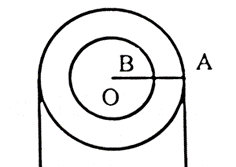
\includegraphics[scale=0.4]{../figs/VN10-2021-PH-TP006-1.png}
		\end{center}
		
	}
	
	\hideall
	{	
		Hai điểm A và B có cùng tốc độ góc nên:
		$$\dfrac{R_\text{B}}{R_\text{A}} = \dfrac{v_\text{B}}{v_\text{A}}$$
		
		Với $R_\text{A} - R_\text{B} = \text{AB} = \SI{10}{cm}$, suy ra
		
		$$R_\text{A} =\SI{15}{cm}$$
		$$\omega=\SI{16}{rad/s}$$
	}
	\item \mkstar{2}
	
	
	{
		Roto trong một tổ máy của nhà máy thủy điện Hòa Bình quay 125 vòng mỗi phút. Hãy tính tốc độ góc của roto này theo đơn vị rad/s.
	}
	
	\hideall
	{	
		Trong 1 giây roto này quay được số vòng là
		
		$$n=\dfrac{125}{60} = \dfrac{25}{12}\ \text{vòng}.$$
		
		Tốc độ góc của roto này là
		
		$$\omega = \dfrac{2\pi n}{t} \approx \SI{13,1}{rad/s}.$$
	}
		\item \mkstar{2}
	
	
	{
		Biết chiều dài kim phút và kim giây của một chiếc đồng hồ lần lượt là $\SI{4}{cm}$ và $\SI{5}{cm}.$ Hãy tính tỉ số chu kì quay của hai kim và  tỉ số độ của đầu kim phút và đầu kim giây.
		
		
	}
	
	\hideall
	{	
		Kim phút quay 1 vòng thì tương ứng là 1 giờ bằng $\SI{3600}{s}$. Chu kỳ quay là $T_1=\SI{3600}{s}$.
		
		Kim giây quay 1 vòng thì tương ứng là 1 phút bằng $\SI{60}{s}$. Vậy chu kỳ là $T_2\SI{60}{s}.$
		
		Tỉ số chu kỳ quay của kim giây và kim phút là 
		
		$$\dfrac{T_2}{T_1} = \dfrac{60}{3600} = \dfrac{1}{60}.$$
		
		Gọi $\omega_1, \omega_2$ lần lượt là tốc độ góc của kim phút và kim giây. $T_1, T_2$ là chu kỳ quay của kim phút và kim giây. 
		
		Tỉ số tốc độ của đầu kim phút và đầu kim giây là:
		
		$$\dfrac{4\omega_1}{5\omega_2} = \dfrac{4}{5} \cdot \dfrac{2\pi}{T_1} \dfrac{T_2}{2\pi} = \dfrac{4}{5} \cdot \dfrac{T_2}{T_1} = \dfrac{1}{75}.$$
		
	}

		\item \mkstar{2}
	
	
	{
		Xét một điểm nằm trên đường xích đạo trong chuyển động tự quay của Trái Đất. Biết bán kính Trái Đất tại xích đạo là $\SI{6400}{km}.$ Hãy tính chu kì chuyển động của điểm đó.
	}
	
	\hideall
	{	
		Trái Đất quay một vòng 24h. Chu kỳ quay của một điểm nằm trên đường xích đạo quanh trục Trái Đất:
		
		$$T = \SI{24}{h} = \SI{86400}{s}.$$
		
	}
	\item \mkstar{2}
	
	
	{
		Xét một điểm nằm trên đường xích đạo trong chuyển động tự quay của Trái Đất. Biết bán kính Trái Đất tại xích đạo là $\SI{6400}{km}.$ Hãy tính tốc độ và tốc độ góc của điểm đó.
	}
	
	\hideall
	{	
		Tốc độ góc của điểm đó là: 
		
		$$\omega = \dfrac{2\pi}{T} = \text{7,3} \cdot 10^{-5}\ \text{rad/s}.$$
		
		Tốc độ của điểm đó là:
		
		$$v = \omega r = \SI{467,2}{m/s}.$$
	}
		\item \mkstar{2}
	
	
	{
		Một đồng hồ điểm 3h30ph. Hãy tính góc quay từ vị trí 12h đến vị trí của kim phút và kim giờ. 
	}
	
	\hideall
	{	
		Kim phút: Tại 12h kim phút chỉ số 12, đến 3h30p thì kim phút chỉ số 6, ta thấy kim phút đi được một nửa vòng tròn.($180^\circ$)
		
		Kim giờ: 1 giờ, kim giờ quay được 1 góc $30^\circ$. 
		
		Từ 12h đến 3h30p tương ứng là 3,5h thì kim giờ quay được 1 góc là 3,5$\cdot 30^\circ = 105^\circ.$
		
		
	}
	\item \mkstar{2}
	
	
	{
		Một em bé cưỡi ngựa gỗ trên sàn quay, ở cách trục quay $\SI{2,1}{m}$. Tốc độ góc của sàn quay là $\SI{0,42}{rad/s}$. Tính tốc độ của ngựa gỗ.
	}
	
	\hideall
	{	
		Tốc độ của ngựa:
		
		$$v = \omega r = \SI{0,882}{m/s}.$$
	}
\end{enumerate}